
In order to conduct a multi-strand analysis with a quench velocity-based approach, one should estimate the quench velocity for varying values of magnetic field that can be found in the magnet. In the previous section, it was concluded that the maximum magnetic field in the skew quadrupole equals $B=3~\text{T}$ and occurs at the initial value of current, $I=86~\text{A}$. As current drops during the discharge, the quench velocity should also decrease because of a lower amount of energy deposited in the coil. Therefore, there are two main variables that have a direct impact on the quench velocity: $(i)$ magnetic field, $(ii)$ transport current. These two parameters are examined in 1D standard simulations with geometries of a relatively short length. 

\subsection{Update of Skew Quadrupole Geometry}
\label{subsection:update_skew_quadrupole_geometry}

In order to model the skew quadrupole with the highest possible precision with respect to the measurements, the modelling of an insulated strand is reformulated in this chapter. Fig.~\ref{fig: 1d_strand_geometry_with_heat_capacity} presents a new 1D+1D model representing a three-dimensional strand. In the~right picture, the nodes marked in red are modelled with the LINK33 element and the strand marked in yellow -- with LINK68. The blue points represent MASS71 elements including an~additional thermal capacity in the strand. MASS71 is a point element having temperature as a degree of freedom characterised by a negligible thermal resistance~\cite{ansys_element_manual}. LINK68 has the material properties of the composite strand whereas both LINK33 and MASS71 -- of G10. The main reason for a change is that, in reality, the windings are in a direct contact through their external insulation (marked in red in the left picture of Fig.~\ref{fig: 1d_strand_geometry_with_heat_capacity}) omitting the resin (marked in blue in the left picture of Fig.~\ref{fig: 1d_strand_geometry_with_heat_capacity}). Moreover, the actual volume of resin between the windings becomes a question mark from the design standpoint. In the fabrication process, the insulated strand is wound first and the resin is added separately to a pre-assembled coil. Therefore, including the resin volume in LINK33 elements is too conservative assumption leading to a relatively slow turn-to-turn propagation. The resin thermal capacity can be added with MASS71 elements.

\begin{figure}[H]
    \centering
    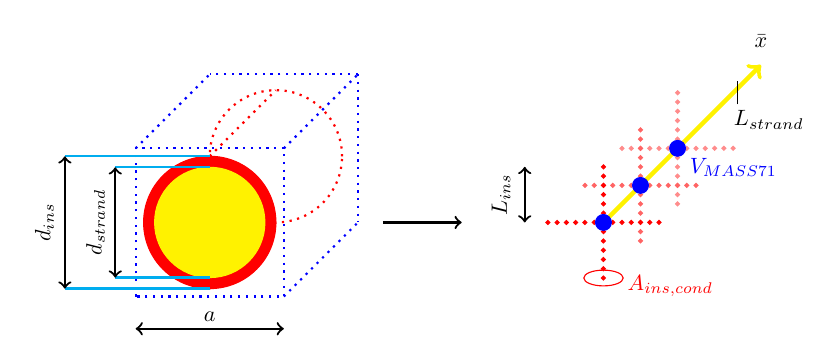
\begin{tikzpicture}[scale = 1]
    
        \draw[thick, blue, dotted] (-0.941,-0.941) rectangle (0.941,0.941);
        \draw[thick, red, dotted] (0.84,0.84) circle (0.7+0.07*2);
        \draw[thick, dotted, red] (0,0.84) -- (0.84,2*0.84);
        \draw[thick, dotted, red] (0,-0.84) -- (0.84,0);
    
        \filldraw[red] (0,0) circle (0.7+0.07*2);
        \filldraw[yellow] (0,0) circle (0.7);
        \draw[thick, cyan] (-0.8*1.5,0.7) -- (0,0.7);
        \draw[thick, cyan] (-0.8*1.5,-0.7) -- (0,-0.7);
        \draw[black, thick, <->] (-0.75*1.6,0.7) -- (-0.75*1.6,-0.7);
        \node[scale = 0.8, rotate=90] at (-1.45, 0) {$d_\text{strand}$};
        
        \draw[thick, cyan] (-0.8*2.3,0.84) -- (0,0.84);
        \draw[thick, cyan] (-0.8*2.3,-0.84) -- (0,-0.84);
        \draw[black, thick, <->] (-0.8*2.3,0.84) -- (-0.8*2.3,-0.84);
        \node[scale = 0.8, rotate=90] at (-2.1, 0) {$d_\text{ins}$};
        \draw[thick, dotted, blue] (0.941,0.941) -- (2*0.941,2*0.941);
        \draw[thick, dotted, blue] (-0.941,0.941) -- (0,2*0.941);
        \draw[thick, dotted, blue] (0.941,-0.941) -- (2*0.941,0);
        \draw[thick, dotted, blue] (2*0.941,2*0.941) -- (2*0.941,0);
        \draw[thick, dotted, blue] (2*0.941,2*0.941) -- (0,2*0.941);

        \node[scale = 0.8] at (0, -1.2) {$a$};
        \draw[thick,<->] (-0.941,-0.9*1.5) -- (0.941,-0.9*1.5);
        
        % ellipse for insulation area
        \draw[red] (5.0,-5.646/8) ellipse (0.25cm and 0.1cm);
        \node[scale = 0.8, red] at (5.85, -5.646/8-0.1) {$A_\text{ins,cond}$};
        % third insulation layer
        \definecolor{red_third_layer}{RGB}{255,140,140}
        \foreach \x in {-5.646,-4.705,...,5.646} 
            \filldraw[red_third_layer] (5.0+2*0.4705,\x/8+2*0.4705) circle (0.025);
        \foreach \x in {-5.646,-4.705,...,5.646} 
            \filldraw[red_third_layer] (5.0+\x/8+2*0.4705,2*0.4705) circle (0.025);
        % second insulation layer
        \definecolor{red_second_layer}{RGB}{255,100,100}
        \foreach \x in {-5.646,-4.705,...,5.646} 
            \filldraw[red_second_layer] (5.0+0.4705,\x/8+0.4705) circle (0.025);
        \foreach \x in {-5.646,-4.705,...,5.646} 
            \filldraw[red_second_layer] (5.0+\x/8+0.4705,0.4705) circle (0.025);
        % first insulation layer
        \definecolor{red_first_layer}{RGB}{255,0,0}
        \foreach \x in {-5.646,-4.705,...,5.646} 
            \filldraw[red_first_layer] (5.0,\x/8) circle (0.025);
        \foreach \x in {-5.646,-4.705,...,5.646} 
            \filldraw[red_first_layer] (5.0+\x/8,0) circle (0.025);
        % strand nodes
        \draw[ultra thick, yellow, ->] (5.0,0) -- (7.0,2.0);
        \foreach \t in {0.0,0.4705,...,1.4115}
            \filldraw[blue] (5.0+\t,\t) circle (0.1);
        \node[scale = 0.8] at (7.1, 1.3) {$L_\text{strand}$};    
        \node[scale = 0.8] at (7, 2.3) {$\bar x$};    
        \draw[thin] (6.7,1.5) -- (6.7,1.8);
        \draw[thick, black, <->] (4,0) -- (4,5.646/8);
        \node[scale = 0.8, rotate=90] at (3.7, 5.646/16) {$L_\text{ins}$}; 
        % draw arrow
        \draw[thick, black, ->] (2.2,0) -- (3.2,0);
        
        \node[blue, scale = 0.8] at (6.65, 0.7) {$V_\text{MASS71}$}; 
        
    \end{tikzpicture}
    \caption{3-dimensional transformation of a 1D+1D strand domain in ANSYS.}
    \label{fig: 1d_strand_geometry_with_heat_capacity}
\end{figure}


This time, the insulation cross-sectional area $A_\text{ins}$ only takes into account the external insulation layer marked in red as
\begin{equation}
    A_\text{ins} = \frac{\pi}{4} \left( d^2_\text{ins} - d^2_\text{strand} \right),
    \label{eqn:new_cross_sectional_area_insulation}
\end{equation}
where $d_\text{ins}$ -- strand diameter with insulation, $d_\text{strand}$ -- strand diameter. Then, the average perimeter should be calculated as
\begin{equation}
    p_\text{avg} =  \frac{\pi}{2} \left( d_\text{ins} + d_\text{strand} \right).
    \label{eqn:new_average_perimeter}
\end{equation}
By combining (\ref{eqn:new_cross_sectional_area_insulation}) and (\ref{eqn:new_average_perimeter}) with (\ref{eqn:equivalent_insulation_length}) one can obtain an equivalent insulation length $L_\text{ins}$. The conduction area $A_\text{ins, cond}$ is calculated as 
\begin{equation}
    A_\text{ins, cond} = \frac{1}{4}~\frac{ A_\text{ins} ~ L_{winding}}{L_\text{ins}}~\frac{1}{n_\text{divisions, winding}}~c_\text{area},
    \label{eqn:new_equivalent_insulation_element_area}
\end{equation}
where $n_\text{divisions, winding}$ -- number of divisions applied along the winding, $c_\text{area}$ -- area coefficient, $L_\text{winding}$ -- straight winding lengths of the coil calculated as
\begin{equation}
    L_\text{winding} = 2~(d+e),
\end{equation}
where the parameters $d$ and $e$ are presented in Fig.~\ref{fig: winding_length_in_skew_quad}. The curvature lengths are not taken into account because they vary with an increasing number of a winding layer.

\begin{figure}[H]
    \centering
    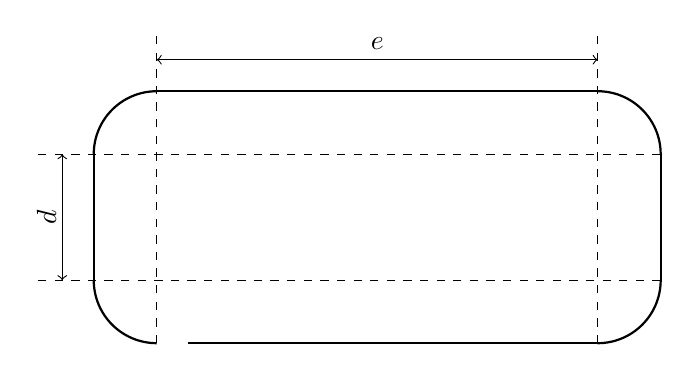
\begin{tikzpicture}[scale = 0.8]
    
        \draw[thick] (0.5,0) -- (7,0);
        \draw[thick] (7,0) arc (-90:0:1);
        \draw[thick] (8,1) -- (8,3);
        \draw[thick] (8,3) arc (0:90:1);
        \draw[thick] (7,4) -- (0,4);
        \draw[thick] (0,4) arc (-270:-180:1);
        \draw[thick] (-1,3) -- (-1,1);
        \draw[thick] (-1,1) arc (-180:-90:1);
        
        \draw[dashed] (0,0) -- (0,5);
        \draw[dashed] (7,0) -- (7,5);
        \draw[dashed] (8,1) -- (-2,1);
        \draw[dashed] (8,3) -- (-2,3);
        
        \draw[<->] (0,4.5) -- (7,4.5);
        \draw[<->] (-1.5,1) -- (-1.5,3);
        
        \node[scale = 1.0] at (3.5,4.75) {$e$};
        \node[scale = 1.0, rotate=90] at (-1.75,2) {$d$};
        
    \end{tikzpicture}
    \caption{Top view of one winding of a high-order corrector geometry.}
    \label{fig: winding_length_in_skew_quad}
\end{figure}

One can observe that Equation~(\ref{eqn:new_equivalent_insulation_element_area}) is similar to (\ref{eqn:equivalent_insulation_element_area}) without taking into consideration $c_\text{area}$. If $c_\text{area} = 1$, the entire insulation volume is packed in the LINK33 elements. If $c_\text{area} < 1$, the remainder of the insulation volume is added to the volume of point MASS71 elements. The reduction of $c_\text{area}$ serves for limiting the contact area between the neighbouring wires and, thus, the heat transfer across the insulation. The volume of a point MASS71 element is calculated as 
\begin{equation}
    V_\text{MASS71} = \frac{\left( a^2 - \frac{\pi d_\text{ins}^2}{4} \right) L_\text{winding}}{n_\text{nodes, winding}}~c_\text{volume} + L_\text{ins}~A_\text{ins, cond} ~ \left( 1-c_\text{area} \right),
    \label{eqn:mass71_volume_element}
\end{equation}
where $c_\text{volume}$ -- resin packing coefficient. If $c_\text{volume} = 0$, no resin is taken into consideration, whereas if $c_\text{volume} = 1$, the entire resin volume is analysed.

\subsection{Quench Velocity Map Based on Standard Analyses}

In this section, a set of 16 standard ANSYS analyses with varying magnetic field and current is conducted. As presented in Fig.~\ref{table: quench_velocity_map_input_parameters_geometry}, a half metre-long winding is used. It is important to mention that the winding length $L_\text{winding}$ refers to a straight strand from Fig.~\ref{fig: 1d_strand_geometry} defined as $L_\text{strand}$. The~model analyses a strand with insulation without resin. The~number of nodes in the longitudinal direction equals $n_\text{nodes, winding}=500$ that corresponds to the mesh size of 1~mm. 20 nodes across the~insulation layer corresponds to the transverse mesh size of 3.5~$\upmu \text{m}$. The mesh size of all dimensions was taken from the reference solution with insulation deduced in Chapter~\ref{chapter:quench_velocity_benchmarking}. Since, the insulation length is shorter in this section because no resin is analysed, the insulation mesh size is even more accurate. 

\begin{table}[H]
    \caption{Geometry input parameters.} 
    \vspace{-1.em} 
    \fontsize{10}{10}
    \selectfont 
    \renewcommand{\arraystretch}{1.5}
    \begin{center}
        \begin{tabular}{ ccc }  
        \hline
        parameter & value & unit \\
        \hline
        $L_\text{winding}$ & 0.5 & [m] \\ 
        $L_\text{ins}$ & 0.07 & [mm] \\
        $c_\text{area}$ & 1.0 & [-] \\
        $c_\text{volume}$ & 0.0 & [-] \\
        $n_\text{nodes, winding}$ & 500 & [-] \\ 
        $n_\text{nodes, insulation}$ & 20 & [-] \\
        \hline 
        \end{tabular}
    \end{center}  
     \label{table: quench_velocity_map_input_parameters_geometry} 
 \end{table}

Table~\ref{table: quench_velocity_map_input_parameters} shows input parameters for the standard analysis. They are mainly based on the simulations conducted in previous chapters. The initial temperature $T_\text{init}$ corresponds to the bath temperature of the measured magnet.

\begin{table}[H]
    \caption{Input parameters for boundary and initial conditions.} 
    \vspace{-1.em} 
    \fontsize{10}{10}
    \selectfont 
    \renewcommand{\arraystretch}{1.5}
    \begin{center}
        \begin{tabular}{ ccc }  
        \hline
        parameter & value & unit \\
        \hline
        $I$ & 26, 46, 66, 86 & [A] \\
        $B$ & 0, 1, 2, 3 & [T] \\
        $T_\text{init}$ & 4.3 & [K] \\
        $T_\text{max}$ & 20.0 & [K] \\
        $L_\text{quench, init}$ & 0.1 & [m] \\ 
        $\alpha$ & 0.223 & [m] \\   
        $t_\text{total}$ & 0.1 & [s] \\
        time step range & $[10, 100]$ & $[\upmu \text{s}]$ \\
        \hline 
        \end{tabular}
    \end{center}  
     \label{table: quench_velocity_map_input_parameters} 
 \end{table}

The initial temperature profile presented in Fig.~\ref{fig: init_gauss_temp_distr_quench_velocity} is calculated based on~(\ref{eqn: gaussian_temp_ic}).

\begin{figure}[H]
\centering
    \begin{tikzpicture}
        \begin{axis}[
          no markers,
          width=0.6\linewidth, 
          height = 4.0cm,
          xlabel={$L_\text{winding},~\text{m}$},
          ylabel={$T,~\text{K}$},
          xmin=0.0,
          ymin=0.0,
          xmax=0.5,
          xtick= {0,0.1,0.2,0.3,0.4,0.5}
          ]
          \addplot table[x=position,y=temperature,col sep=comma] {sections/skew_quad_q_det/figures/v_quench_map/init_gauss_profile.csv}; 
        \end{axis}
    \end{tikzpicture}
    \caption{Initial Gaussian temperature profile.}
    \label{fig: init_gauss_temp_distr_quench_velocity}
\end{figure}

In the first instants of the quench analysis, the quench velocity is usually higher because the bell shape of the Gaussian profile in Fig~\ref{fig: init_gauss_temp_distr_quench_velocity} relaxes longitudinally. However, there is a moment in the simulations when the heat generation during quench becomes the main reason for the quench to propagate. At that moment, the quench velocity stabilises and becomes relatively constant. The quench velocity was calculated at each time window of $\Delta t=10~\text{ms}$. It was assumed in the analyses that the quench velocity stabilises if it does not vary by more than 0.1~m/s. If this condition was met, the analysis was finished and the value of quench velocity was saved. Fig.~\ref{fig: v_quench_map_current_b_field} presents quench velocity values as a function of magnetic field and current. 

\begin{figure}[H]
\centering
    \begin{tikzpicture}
        \begin{axis}[
          width=0.7\linewidth, 
          height = 5.5cm,
          xlabel={$B$, $\text{T}$},
          ylabel={$v_\text{quench}$, $\frac{\text{m}}{\text{s}}$},
          xmin=0.0,
          xmax=3.0,
          ymin=0.0,
          ymax=6.0,
          legend pos = north west
          ]
          \addplot[green, mark=*] table[x=B_field,y=I_86,col sep=comma] {sections/skew_quad_q_det/figures/v_quench_map/v_quench_map.csv};
          \addplot[blue, mark=*] table[x=B_field,y=I_66,col sep=comma] {sections/skew_quad_q_det/figures/v_quench_map/v_quench_map.csv};
          \addplot[red, mark=*] table[x=B_field,y=I_46,col sep=comma] {sections/skew_quad_q_det/figures/v_quench_map/v_quench_map.csv};
          \addplot[black, mark=*] table[x=B_field,y=I_26,col sep=comma] {sections/skew_quad_q_det/figures/v_quench_map/v_quench_map.csv};
          \legend{
          $I=86~\text{A}$,
          $I=66~\text{A}$,
          $I=46~\text{A}$,
          $I=26~\text{A}$}
        \end{axis}
    \end{tikzpicture}
    \caption{Quench velocity map as a function of magnetic field and current.}
    \label{fig: v_quench_map_current_b_field}
\end{figure}